\documentclass[conference]{IEEEtran}
\IEEEoverridecommandlockouts
% The preceding line is only needed to identify funding in the first footnote. If that is unneeded, please comment it out.
\usepackage{cite}
\usepackage{amsmath,amssymb,amsfonts}
\usepackage{algorithmic}
\usepackage{graphicx}
\usepackage{textcomp}
\usepackage{xcolor}
\usepackage{comment}
\usepackage{url}

\def\BibTeX{{\rm B\kern-.05em{\sc i\kern-.025em b}\kern-.08em
    T\kern-.1667em\lower.7ex\hbox{E}\kern-.125emX}}

\begin{document}

\title{%
Fog Computing and SDN in IoT Networks\\

\large \emph {This report was prepared for Professor Ahmed Karmouch in partial fulfillment of the requirements for the course ELG7187F Software Defined Networks and Cloud \\ Group 5 \\}
22 Dec 2022

%Survey on the implementation of FOG computing and SDN
%{\footnotesize This report was prepared for Professor Ahmed Karmouch in partial fulfillment of the requirements for the course ELG7187A Software Defined Networks and Cloud}
%\thanks{Identify applicable funding agency here. If none, delete this.}
}

\author{\IEEEauthorblockN{1\textsuperscript{st} Varun Narayana Naik}
\IEEEauthorblockA{\textit{Department of Electrical and Computer Engineering} \\
\textit{University of Ottawa}\\
Ottawa, Canada \\
vnaik041@uottawa.ca \\
300270736
}
\and
\IEEEauthorblockN{2\textsuperscript{st} Nishad Sanjay Vyas}
\IEEEauthorblockA{\textit{Department of Electrical and Computer Engineering} \\
\textit{University of Ottawa}\\
Ottawa, Canada \\
nvyas028@uottawa.ca \\
300267323}





\begin{comment}
\and
\IEEEauthorblockN{3\textsuperscript{rd} Given Namedddd Surname}
\IEEEauthorblockA{\textit{dept. name of organization (of Aff.)} \\
\textit{name of organization (of Aff.)}\\
City, Country \\
email address or ORCID}
\end{comment}

}
\maketitle

\begin{abstract}
In recent times, the Internet of Things (IoT) has seen rapid advancements and subsequently the number of applications has also increased significantly, resulting in new concepts such as smart health, smart cities, and smart homes. These IoT networks require vast amounts of processing and data storage. Generally, cloud computing is used to meet these demands. Although the cloud can provide processing and resources it still faces some challenges. The rising number of IoT devices as well as the distance between the cloud and these devices is an issue since it leads to higher latency, which is an obstacle for real-time applications. Fog computing, which is a highly virtualized paradigm can address these issues by delivering computational resources, data storage and network services closer to the end devices. However, there are issues such as heterogeneity that plague fog computing and to tackle them centralized network control in the form of Software Defined Networking (SDN) is needed. In this paper, we describe SDN-enabled fog computing and its architecture. Then, we present the unique features and advantages of SDN-enabled fog over traditional fog computing. Finally, we have discussed the challenges and solutions currently faced in this paradigm.
\end{abstract}

\begin{IEEEkeywords}
Fog computing, Software Defined Networking, Fog-SDN, Internet of Things
\end{IEEEkeywords}

\section{Introduction}
The   advent of the internet and the rise of smart devices has led to the growth of the Internet of Things (IoT) and hence the IoT revolution. IoT encompasses smart devices and objects that have electronics, software and networking capability that allow inter-device communication \cite{donno}. These devices such as smart vehicles, and smart appliances use the IoT network to exchange data. The scale of growth is estimated to reach 75 billion devices alone,  this means a much larger number of connections are needed to interconnect these devices \cite{vail}. There are a lot of advances being made in computing paradigms. The most well know paradigm is that of cloud computing, providing a centralized approach to enabling computing as a utility and acting as a catalyst for internet services development. But such a centralized paradigm has inevitably led to some limitations and has opened doors for a more decentralized paradigm to computing, one that can address the challenges of latency, bandwidth and anomaly detection. As a result, new approaches have been developed such as fog computing. The decentralized nature itself presents new problems when dealing with routing data among the nodes, hence complex network management and traffic engineering are crucial to reducing the data transmission latency. The idea of Software-defined networking has proven useful in this aspect. In this paper, we refer to the combination of fog and SDN as SDN-enabled fog or fog-SDN.

\subsection{Fog Computing}
Fog computing is a decentralized approach to computing in stark contrast to the centralized nature of traditional cloud computing. A term coined by Cisco \cite{cisco}; Fog computing is defined as the cloud near the network edge closer to the end devices and acts as an intermediary between the IoT and the cloud\cite{donno}. Fog aims to bring computing and data storage closer to IoT devices. Fog computing works in conjunction with the cloud and acts as a bridge between the cloud and IoT devices\cite{verma}. It does not aim to replace cloud computing but rather distributes the resources in all directions in the cloud IoT continuum. It addresses the problems associated with cloud computing such as high latency, bandwidth, location awareness and reliability since the processing power is brought closer to the IoT devices which also provides better access to data storage. This structure can be represented by three layers namely, the IoT device layer, fog layer and cloud layer. While fog handles local data, the cloud handles mainly global data.  The fog network constitutes fog nodes that are low processing-power devices such as servers, devices, or virtual machines. The fog nodes communicate with the IoT devices and form a bridge to the cloud. These nodes can be placed anywhere between the cloud and the IoT devices in the cloud-IoT continuum. These nodes communicate with each other to exchange data and resources. The fog nodes process the real-time data at the edge of the network without sending large amounts of data to the cloud. However, if the processing power of the fog nodes is insufficient, the fog nodes send the data to the cloud for further processing. The presence of numerous fog nodes provides better services to IoT devices compared to cloud data centres; hence fog has more services to offer like lower latency, better bandwidth and location awareness. This has paved the way to support applications such as smart homes, smart healthcare and smart cities which require real-time analysis.

\subsection{Software Defined Networking (SDN)}
Software-defined networking is a paradigm where the data plane is separated from the control plane and a central controller governs the network behaviour \cite{benz}. The aim is to form a centralized intelligence having a global view of the network which not only allows easier network management but rather better network security. The network control logic is implemented by the controller and is separated from the forwarding process where the network devices perform packet forwarding. 

Being software in nature, SDN allows new changes to be made to the network easily using a software program compared to using fixed commands in the network devices. Due to its centralized approach, SDN can make traffic forwarding decisions from a single controller and thus removes the need to individually configure each network device to change network behaviour\cite{hkim}. The conventional hardware-based network architecture is error-prone and has complex network control. Any failure results in expensive and time-consuming repairs. Using a software-based architecture removes the need for highly skilled network engineers. The process of managing a network becomes easier since the control plane only deals with traffic management and network topology, hence can be used to control fog nodes and based on the configurations in the control plane, the data plane manages the flow of traffic in the fog nodes. 

The separation of layers allows the network providers to distribute the resources using the application layer which also provides services like routing and monitoring. They can configure the network policies using the control plane where all the control logic resides and set up hardware routers and nodes using the data plane which is formed by the interconnected forwarding devices.  The protocols used to provide communication between the controller and the forwarding devices are known as southbound Application Programming Interfaces (APIs). One such is the OpenFlow API, which defines the flow rules used by network devices. Whereas northbound APIs are used to connect the applications and the control plane. Thus Software-defined networking enables the concurrent update of network resources as per the application and data scaling.

This paper makes contributions such as: We describe what is fog computing. We give a brief description of the working of fog computing and how it compares with cloud computing as well as how it works in conjunction with cloud computing. Next, we talk about what Software-defined networking is and how it is used to handle networking when compared to traditional hardware methods. We discuss how SDN can be used for fog computing and how they can complement each other. We see the architecture of such a proposed new paradigm. Furthermore, we describe what are its characteristics and benefits for use in IoT networks. We also present a few challenges that add limitations to reaching the full potential of fog computing which are solved using SDN.

The outline of the paper is as follows. Section II defines the architecture of SDN-enabled fog computing. It provides details about each component. Section III outlines the advantages and characteristics of SDN-enabled fog that make it useful for IoT networks. Section IV briefly discusses the real-world applications of SDN-enabled fog. Section V discusses the challenges and solutions faced by the SDN-enabled fog domain. Finally, Section VI ends the paper with the conclusion.


\section{Architecture of SDN-Enabled Fog}
\begin{comment}
\begin{figure}[h]
\centerline{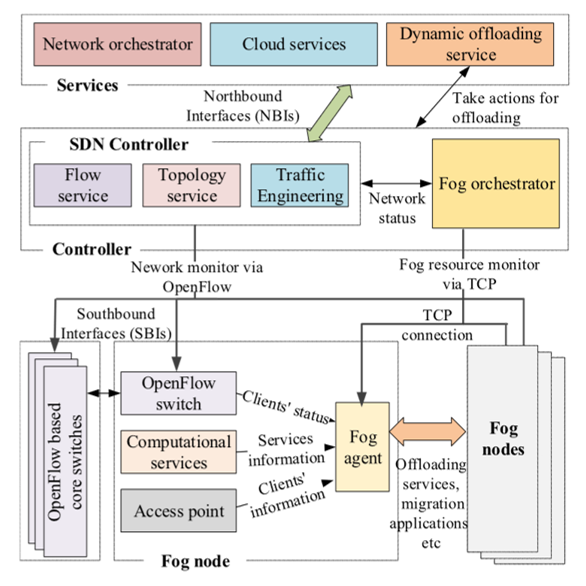
\includegraphics{Images/FOG SDN ARCH.png}}
\caption{Architecture of SDN-enabled Fog}
\label{fog SDN architecture}
\end{figure}
\end{comment}

\begin{figure}[h]
    \centering
    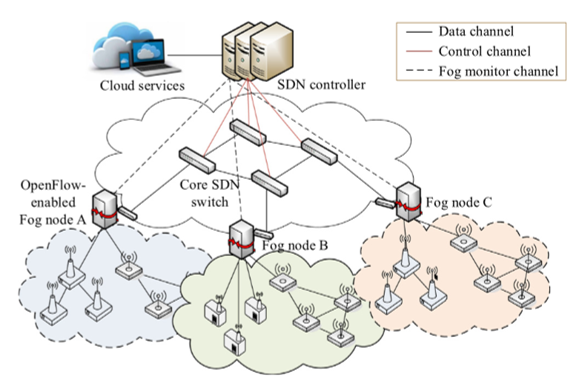
\includegraphics[width=0.5\textwidth]{Images/sdn fog model.png}
    \caption{SDN-Enabled Fog Model}
    \label{fig:fog sdn model}
\end{figure}

The emergence of complex IoT paradigms needs solutions that can handle the latency and resource requirements. Fog computing is a viable solution to this issue as it develops on the existing technology of cloud computing. IoT applications in smart cities, healthcare and industry have strict requirements for latency. This is solved by fog computing by bringing the computing resources and the data storage closer to the IoT devices near the edge. Thus fog computing closes the gap between the IoT paradigm and cloud computing. With the presence of numerous networking elements in the form of fog nodes as discussed earlier, the latency with each node traversed increases, hence it is vital to configure and manage how data is transferred among the network elements to meet the latency needs\cite{herr}. This issue of managing the network flow and traffic is best handled by using Software-defined networking (SDN) as shown by Fig. \ref{fig:fog sdn model}. Moreover, it can help with the scalability and flexibility of the fog network. Hence an SDN-enabled fog is utilised for IoT applications. The Fig. \ref{fig:fog sdn arch} shows the structure of such an SDN-enabled fog. There are mainly four components such as fog nodes, SDN switches, a controller and services.


\begin{figure}[h]
    \centering
    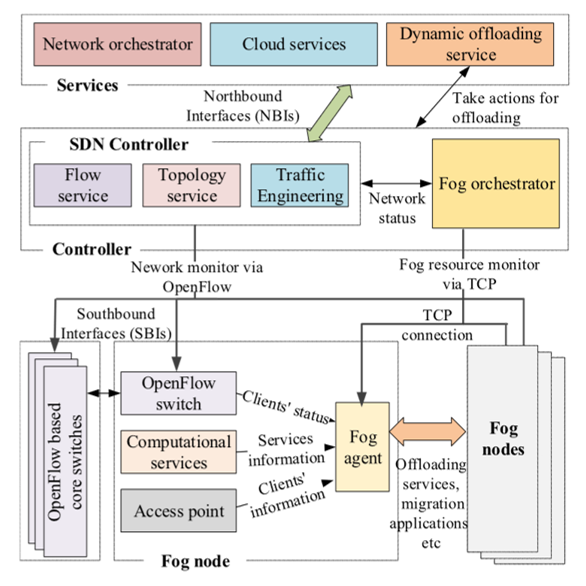
\includegraphics[width=0.5\textwidth]{Images/FOG SDN ARCH.png}
    \caption{Architecture of SDN-Enabled Fog}
    \label{fig:fog sdn arch}
\end{figure}
\subsection{Fog Nodes}
A fog node interacts directly with IoT end devices such as smart watches, thermostats, cameras, mobile phones and so on. It does so using a wireless interface. The fog nodes form the fog domain and it can be comprised of devices such as routers, switches, gateways, computers and set-top boxes\cite{moura}. Each node has a fog agent and several computational services\cite{phan}. The fog nodes communicate with the controller through an SDN core switches. The fog node is connected to the fog orchestrator present within the controller using the fog agent. The purpose of this fog agent is to send vital information about the fog nodes such as the availability and capacity of the computational resources, and hardware specifications which are further used by the various services.

\subsection{SDN Switches}
The SDN switches form the core SDN network. These SDN switches are controlled by an SDN controller\cite{phan}. OpenFlow is used by these switches to communicate with the controller. The controller can change the flow rules in the switches, this lets the controller dynamically control the network. The SDN controller periodically collects information about the network properties such as latency and bandwidth through the switches. The SDN network and the fog nodes are often maintained by one organization in small-scale systems. Whereas, in large-scale systems, these can be handled by multiple organizations working together. 

\subsection{Controller}
The controller is known as the brain of the SDN-enabled fog\cite{benz}. It houses the SDN controller and the fog orchestrator. Some of the well-known SDN controllers are NOX \cite{hu}  and OpenDaylight \cite{med} and one of the well-known fog orchestrators is FORCH \cite{davo}. The SDN controller handles network management and traffic monitoring. It establishes the flow tables and rules as well as the policies for handling the data. The controller helps in abstracting the network complexity. The controller is connected to the services using the northbound APIs. The SDN controller uses the southbound APIs (OpenFlow) to connect with the SDN switches. The controller uses the SDN switches to ensure proper forwarding, fragmentation and reassembly take place. The fog orchestrator handles the fog node operation. The fog agent and SDN switches are used to gain information about the fog nodes and the network. 
 
 \subsection{Services}
This layer consists of applications that can provide various functionalities to the end devices. These services are developed to help the operation of the fog system. The controller uses northbound interfaces such as OpenDaylight to communicate with the topmost layer, the services. The services offered include firewall, quality of service, access control and proxy control. 

\section{Advantages of Fog and SDN}
\subsection{Handling Heterogeneity }
The IoT network is heterogenous in nature due presence of a wide diversity of IoT devices. IoT devices often have different data formats and different protocols for communication information which is also influenced by the presence of legacy devices \cite{qin}. These devices are made up of various types of hardware configurations, protocols, communication technologies and standards. The application of SDN providing network control over the fog enables multiple protocols and devices to be interconnected. Not only does the SDN allow interoperability among various types of fog nodes, but it also enables interoperability between end devices of different types which can be physical or virtual. SDN-enabled fog can handle IoT devices using heterogeneous networks  for communication such Wifi, Bluetooth and ethernet\cite{bed}. Thus SDN-enabled fog computing can provide a platform for these devices of different environments to interoperate with each other. Moreover, various service providers are often used in a large-scale system and SDN-enabled fog computing can effectively handle these different service providers. 

\subsection{Location Awareness}
In SDN-enabled fog, the nodes are not centralized in one location, rather they are distributed in different locations. The SDN, having a global view of the network as well as the fog nodes enables location awareness and geographical distribution of resources\cite{atlam}. The IoT devices are far away from the cloud servers and need real-time communication with the server for computing and resources, but by utilising fog nodes in close proximity and the traffic engineering of SDN, the data can be processed efficiently and closer to the IoT devices. This in turn improves performance by drastically reducing the delays for real-time applications. The services and the applications offered by fog are distributed as well and can be easily accessed by end devices compared to cloud services. Due to the location awareness  of fog-SDN, the location of the fog nodes can be determined accurately\cite{gia}. Hence the presence of fog nodes near the end devices helps determine the location of the end devices easily\cite{zhang}. This is particularly useful for application in smart cities and healthcare as the location can have an impact on the Quality of Service (QoS)\cite{mark}.

\subsection{Network Security and Privacy}
While fog computing has benefits such as latency, fast processing, service allocation and many more, a security issue is associated with them. These fog nodes lack efficient security algorithms, and the data stored in them might get breached by hackers or malicious users. The existing solutions are only partially suitable for IoT devices with limited computational resources. To overcome these security issues \cite{kahva}, fog nodes can be enabled by a centralized SDN controller in the cloud layer and multiple distributed controllers near the edge in the control layer. It works on a master-slave paradigm, wherein the central controller manages the secure communication for all the components in the network. The SDN controllers in the control layers act as a sub-master, providing secure mobility to this architecture and ensuring secure, manageable, and coordinated communication between fog nodes and the cloud. The slaves in this architecture are the devices at the edge of the network, including all the sensors and mobile components. The controller in this network helps reduce the delay time for authentication for communications between fog and cloud, which was very difficult to achieve with just the fog network.

\subsection{Resource and Network Management}
Enabling fog computing with SDN eases communication among the fog nodes to ensure good performance. Fog computing can be beneficial for real-time applications which require low latency and real-time responses, but its network diversity can become challenging to manage. Using SDN controllers in conjunction with fog nodes can provide low latency along with efficient resource and network management. For smart grids in Wireless Body Area Networks (WBANs)\cite{ren}, a three-layered architecture is used for efficient resource management. The architecture's bottom layer consists of all the IoT sensors responsible for generating the data. The middle layer, or the second layer, has fog nodes which comprise intelligent meters and servers, these servers are responsible for collecting data generated by the first layer. In the third layer, there is an SDN controller that manages all the fog nodes. The SDN controller manages data forwarding by using the shortest path algorithm and three types of path recoveries in case any failure occurs during data transmission. Similarly, for the Internet of Vehicles (IoV), the same architecture can have five layers for better Central Processing Unit (CPU) utilization in case it is overloaded or under-loaded \cite{alomari}.


\section{Applications}
Fog computing can have various applications in different domains, such as real-time traffic regulation in smart cities, garbage truck routing using sensors in garbage bins, real-time video processing for surveillance systems and many more. Although it has many applications with increases in network size and number of devices, there are some limitations to it, such as high latency and node overloading, which can be tackled by utilizing an SDN controller, which will be discussed in the next section.

Smart healthcare is one of the significant applications of fog computing, which is being improved with the help of SDN. In e-healthcare, fog-SDN ensures the Quality-of-Service parameters like bandwidth, latency, higher throughput, and less packet loss while ensuring the privacy and the security of the patient’s sensitive information is secured. This is made possible by the centralized SDN controller, and the flow rules designed by these controllers and switches. Based on these flow rules, the switches decide to send the packets to the cloud or to process them at the edge; further discussion about similar implementation is presented in the next section.

\begin{figure}[h]
    \centering
    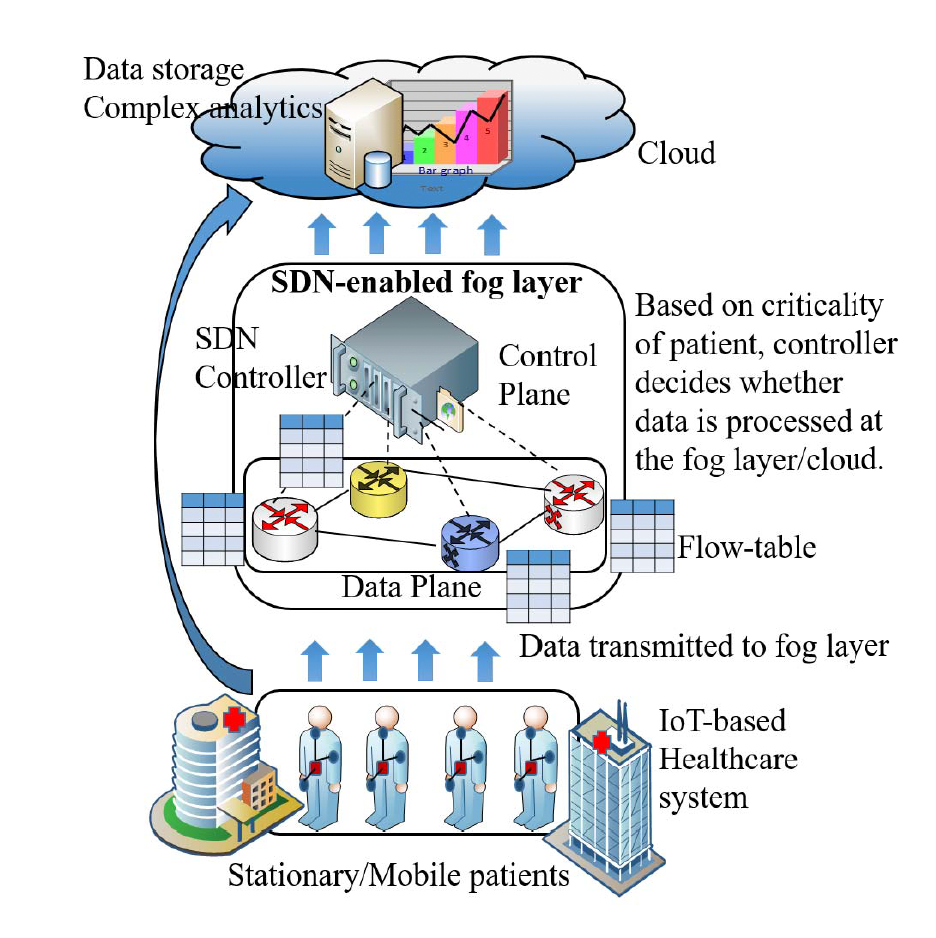
\includegraphics[width=0.5\textwidth]{Images/latency.png}
    \caption{Architecture of SDN-Enabled Fog}
    \label{fig:latency}
\end{figure}

\section{Challenges and Solutions}
\subsection{Latency}
In applications concerning healthcare data, the transmission of packets is very time critical. While transmitting the data to the server, factors such as throughput, latency, and loss of packets can affect the network's performance. These issues must be addressed to process information in real time with less delay while efficiently utilizing the network's available resources. The proposed architecture \cite{roy} considers patients' health conditions and determines a Criticality Index (CI) to prioritize the tasks in the network. 

In Fig. \ref{fig:latency}, the architecture is divided into three parts, a traditional wireless-based network consists of all the sensor nodes that collect the patient's information. The SDN-enabled fog layer consists of a control plane with an SDN controller and the OpenFlow switches in the data plane with their flow rules. Finally, a cloud layer comprises data centers for storing patients' information, such as Electronic Medical Images (EMI), Electronic Medical Records (EMR) and Electronic Health Records (EHR) for complex analytics. Whenever OpenFlow switches receive data packets from the WBAN, they determine their criticality index, which is divided into subranges to consider cases in which patients' conditions might be deteriorating quickly. Based on the criticality index, the OpenFlow switches decide whether to send the data to the cloud or to process it at the fog nodes. Utility values such as energy consumption and bandwidth are also considered. If no fog nodes are available, the controller will find newly updated nodes and update the flow table while recomputing the utility values. Finally, after the task completion, the fog node sends a signal to the SDN controller to update the flow table and utility values. Furthermore, to reduce latency, this number of flow rules is reduced by replacing the most used flow rule with the least used one.


\subsection{Task Offloading}
Even though fog computing works well in reducing the latency between the end devices and the cloud center, the fog node can get overloaded due to a surge in requests from the IoT devices. For issues such as this, an effective task-offloading technique must be implemented in the fog nodes \cite{phan}. SDN-based fog computing networks can dynamically offload the tasks to improve the bandwidth between end devices and the cloud center. Fig. \ref{fig:task offloading} depicts the offloading scheme used by the fog-SDN network to efficiently manage the incoming task requests and select the optimal node for its processing. When a fog node is overloaded, it sends a request for offloading the task to the fog orchestrator, and this request contains resource requirements. Node selection is made in two steps; in the first step, the offloading service starts a search for all the available optimal nodes capable of handling the requested task. The second step ranks all these nodes based on the network condition and computational resources. Dividing this process into two steps improves the running time because the first step reduces the number of nodes which will then be input for step 2. Finally, the node accepting the offload request is selected based on the least communication cost compared to other fog nodes. Any algorithm can be used and applied in the OpenFlow switches for choosing the optimal routing path for the task offloading.

\begin{figure}[h]
    \centering
    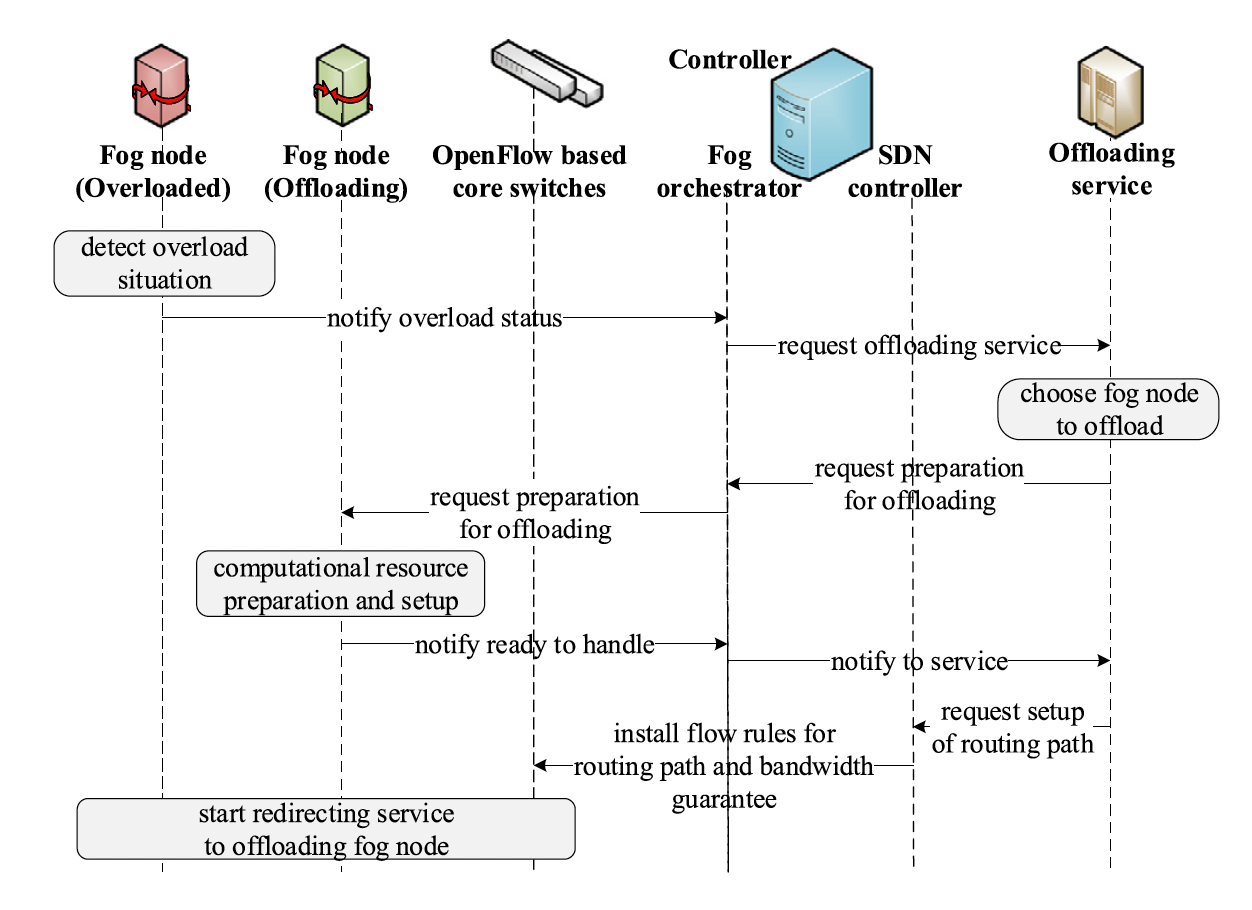
\includegraphics[width=0.5\textwidth]{Images/task_offloading.png}
    \caption{Sequence of Task Offloading in Fog-SDN}
    \label{fig:task offloading}
\end{figure}

\section{Conclusion}
Fog computing along with SDN forms a bridge between the cloud and the IoT end devices and helps support real-time applications. In this paper, we have described SDN-enabled fog which is an architecture that combines the advantages of fog computing and SDN for IoT devices. We looked at how fog computing can be beneficial for IoT applications and how the performance can be further improved by using SDN. We also described the advantages of fog-SDN such as interoperability to tackle heterogeneity, location awareness to deal with the vast size of IoT, network management to handle the resources efficiently and network security to deal with data intrusion. We have also mentioned how fog-SDN can be used for various applications such as smart cities and smart healthcare. Finally, we have identified the challenges such as the overloading of fog nodes and high latency in time-sensitive applications. We have also detailed the solutions to these challenges that can be achieved by using SDN with fog computing. 
\\

This paper covers various aspects of fog computing and SDN by providing descriptions of the advantages, applications and challenges. For future work, we would like to delve deeper into the research focusing on the advantages of fog-SDN.


\begin{thebibliography}{00}

\bibitem{donno} M. De Donno, K. Tange, and N. Dragoni, “Foundations and evolution of modern computing paradigms: Cloud, IOT, Edge, and Fog,” IEEE Access, vol. 7, pp. 150936–150948, 2019. 
\bibitem{vail} L. S. Vailshery, “IOT devices installed Base Worldwide 2015-2025,” Statista, 27-Nov-2016. [Online]. Available: https://www.statista.com/statistics/471264/iot-number-of-connected-devices-worldwide/. [Accessed: 17-Dec-2022]. 
\bibitem{cisco}“What is edge computing?,” Cisco, 20-Oct-2021. [Online]. Available: https://www.cisco.com/c/en/us/solutions/computing/what-is-edge-computing.html. [Accessed: 17-Dec-2022].
\bibitem{verma}P. Verma and S. K. Sood, “Fog assisted-IOT enabled patient health monitoring in Smart Homes,” IEEE Internet of Things Journal, vol. 5, no. 3, pp. 1789–1796, 2018. 
\bibitem{benz}K. Benzekki, A. El Fergougui, and A. Elbelrhiti Elalaoui, “Software-defined networking (SDN): A survey,” Security and Communication Networks, vol. 9, no. 18, pp. 5803–5833, 2016. 
\bibitem{hkim}H. Kim and N. Feamster, “Improving network management with software defined networking,” IEEE Communications Magazine, vol. 51, no. 2, pp. 114–119, 2013. 
\bibitem{herr}J. L. Herrera, J. Galan-Jimenez, L. Foschini, P. Bellavista, J. Berrocal, and J. M. Murillo, “QoS-aware fog node placement for intensive IOT applications in SDN-fog scenarios,” IEEE Internet of Things Journal, vol. 9, no. 15, pp. 13725–13739, 2022. 
\bibitem{moura}C. Mouradian, D. Naboulsi, S. Yangui, R. H. Glitho, M. J. Morrow and P. A. Polakos, "A Comprehensive Survey on Fog Computing: State-of-the-Art and Research Challenges," in IEEE Communications Surveys \& Tutorials, vol. 20, no. 1, pp. 416-464, Firstquarter 2018, doi: 10.1109/COMST.2017.2771153.
\bibitem{phan}L.-A. Phan, D.-T. Nguyen, M. Lee, D.-H. Park, and T. Kim, “Dynamic fog-to-fog offloading in SDN-based Fog Computing Systems,” Future Generation Computer Systems, vol. 117, pp. 486–497, 2021. 
\bibitem{hu}F. Hu, Q. Hao, and K. Bao, “A survey on software-defined network and openflow: From concept to implementation,” IEEE Communications Surveys \& Tutorials, vol. 16, no. 4, pp. 2181–2206, 2014. 
\bibitem{med}J. Medved, R. Varga, A. Tkacik, and K. Gray, “OpenDaylight: Towards a model-driven SDN controller architecture,” Proceeding of IEEE International Symposium on a World of Wireless, Mobile and Multimedia Networks 2014, 2014. 
\bibitem{davo}G. Davoli, D. Borsatti, D. Tarchi and W. Cerroni, "FORCH: An Orchestrator for Fog Computing service deployment," 2020 IFIP Networking Conference (Networking), 2020, pp. 677-678.
\bibitem{qin}Z. Qin, G. Denker, C. Giannelli, P. Bellavista, and N. Venkatasubramanian, “A software defined networking architecture for the internet-of-things,” 2014 IEEE Network Operations and Management Symposium (NOMS), 2014. 
\bibitem{bed}I. Bedhief, M. Kassar, and T. Aguili, “SDN-based architecture challenging the IOT heterogeneity,” 2016 3rd Smart Cloud Networks \& Systems (SCNS), 2016. 
\bibitem{atlam}H. Atlam, R. Walters, and G. Wills, “Fog computing and the internet of things: A Review,” Big Data and Cognitive Computing, vol. 2, no. 2, p. 10, 2018. 
\bibitem{gia}T. N. Gia, M. Jiang, A.-M. Rahmani, T. Westerlund, P. Liljeberg, and H. Tenhunen, “Fog computing in healthcare internet of things: A case study on ECG feature extraction,” 2015 IEEE International Conference on Computer and Information Technology; Ubiquitous Computing and Communications; Dependable, Autonomic and Secure Computing; Pervasive Intelligence and Computing, 2015. 
\bibitem{zhang}J. Ni, K. Zhang, X. Lin, and X. Shen, “Securing fog computing for internet of things applications: Challenges and solutions,” IEEE Communications Surveys \& Tutorials, vol. 20, no. 1, pp. 601–628, 2018. 
\bibitem{mark}A. Markus, J. D. Dombi, and A. Kertesz, “Location-aware task allocation strategies for IOT-fog-cloud environments,” 2021 29th Euromicro International Conference on Parallel, Distributed and Network-Based Processing (PDP), 2021. 
\bibitem{kahva}S. Kahvazadeh, V. B. Souza, X. Masip-Bruin, E. Marn-Tordera, J. Garcia, and R. Diaz, “Securing combined fog-to-cloud system through SDN approach,” Proceedings of the 4th Workshop on CrossCloud Infrastructures \& Platforms - Crosscloud'17, 2017. 
\bibitem{ren}J. Ren, J. Li, H. Liu, and T. Qin, “Task offloading strategy with emergency handling and blockchain security in SDN-empowered and fog-assisted healthcare IOT,” Tsinghua Science and Technology, vol. 27, no. 4, pp. 760–776, 2022.
\bibitem{alomari}A. Alomari, S. K. Subramaniam, N. Samian, R. Latip, and Z. Zukarnain, “Resource Management in SDN-based Cloud and SDN-based Fog Computing: Taxonomy study,” Symmetry, vol. 13, no. 5, p. 734, 2021.
\bibitem{roy}C. Roy, R. Saha, S. Misra, and D. Niyato, “Soft-Health: Software-defined fog architecture for IOT applications in Healthcare,” IEEE Internet of Things Journal, vol. 9, no. 3, pp. 2455–2462, 2022.



\end{thebibliography}
\vspace{12pt}
\begin{comment}
\section{Ease of Use}

\subsection{Maintaining the Integrity of the Specifications}

The IEEEtran class file is used to format your paper and style the text. All margins, 
column widths, line spaces, and text fonts are prescribed; please do not 
alter them. You may note peculiarities. For example, the head margin
measures proportionately more than is customary. This measurement 
and others are deliberate, using specifications that anticipate your paper 
as one part of the entire proceedings, and not as an independent document. 
Please do not revise any of the current designations.

\section{Prepare Your Paper Before Styling}
Before you begin to format your paper, first write and save the content as a 
separate text file. Complete all content and organizational editing before 
formatting. Please note sections \ref{AA}--\ref{SCM} below for more information on 
proofreading, spelling and grammar.

Keep your text and graphic files separate until after the text has been 
formatted and styled. Do not number text heads---{\LaTeX} will do that 
for you.

\subsection{Abbreviations and Acronyms}\label{AA}
Define abbreviations and acronyms the first time they are used in the text, 
even after they have been defined in the abstract. Abbreviations such as 
IEEE, SI, MKS, CGS, ac, dc, and rms do not have to be defined. Do not use 
abbreviations in the title or heads unless they are unavoidable.

\subsection{Units}
\begin{itemize}
\item Use either SI (MKS) or CGS as primary units. (SI units are encouraged.) English units may be used as secondary units (in parentheses). An exception would be the use of English units as identifiers in trade, such as ``3.5-inch disk drive''.
\item Avoid combining SI and CGS units, such as current in amperes and magnetic field in oersteds. This often leads to confusion because equations do not balance dimensionally. If you must use mixed units, clearly state the units for each quantity that you use in an equation.
\item Do not mix complete spellings and abbreviations of units: ``Wb/m\textsuperscript{2}'' or ``webers per square meter'', not ``webers/m\textsuperscript{2}''. Spell out units when they appear in text: ``. . . a few henries'', not ``. . . a few H''.
\item Use a zero before decimal points: ``0.25'', not ``.25''. Use ``cm\textsuperscript{3}'', not ``cc''.)
\end{itemize}

\subsection{Equations}
Number equations consecutively. To make your 
equations more compact, you may use the solidus (~/~), the exp function, or 
appropriate exponents. Italicize Roman symbols for quantities and variables, 
but not Greek symbols. Use a long dash rather than a hyphen for a minus 
sign. Punctuate equations with commas or periods when they are part of a 
sentence, as in:
\begin{equation}
a+b=\gamma\label{eq}
\end{equation}

Be sure that the 
symbols in your equation have been defined before or immediately following 
the equation. Use ``\eqref{eq}'', not ``Eq.~\eqref{eq}'' or ``equation \eqref{eq}'', except at 
the beginning of a sentence: ``Equation \eqref{eq} is . . .''

\subsection{\LaTeX-Specific Advice}

Please use ``soft'' (e.g., \verb|\eqref{Eq}|) cross references instead
of ``hard'' references (e.g., \verb|(1)|). That will make it possible
to combine sections, add equations, or change the order of figures or
citations without having to go through the file line by line.

Please don't use the \verb|{eqnarray}| equation environment. Use
\verb|{align}| or \verb|{IEEEeqnarray}| instead. The \verb|{eqnarray}|
environment leaves unsightly spaces around relation symbols.

Please note that the \verb|{subequations}| environment in {\LaTeX}
will increment the main equation counter even when there are no
equation numbers displayed. If you forget that, you might write an
article in which the equation numbers skip from (17) to (20), causing
the copy editors to wonder if you've discovered a new method of
counting.

{\BibTeX} does not work by magic. It doesn't get the bibliographic
data from thin air but from .bib files. If you use {\BibTeX} to produce a
bibliography you must send the .bib files. 

{\LaTeX} can't read your mind. If you assign the same label to a
subsubsection and a table, you might find that Table I has been cross
referenced as Table IV-B3. 

{\LaTeX} does not have precognitive abilities. If you put a
\verb|\label| command before the command that updates the counter it's
supposed to be using, the label will pick up the last counter to be
cross referenced instead. In particular, a \verb|\label| command
should not go before the caption of a figure or a table.

Do not use \verb|\nonumber| inside the \verb|{array}| environment. It
will not stop equation numbers inside \verb|{array}| (there won't be
any anyway) and it might stop a wanted equation number in the
surrounding equation.

\subsection{Some Common Mistakes}\label{SCM}
\begin{itemize}
\item The word ``data'' is plural, not singular.
\item The subscript for the permeability of vacuum $\mu_{0}$, and other common scientific constants, is zero with subscript formatting, not a lowercase letter ``o''.
\item In American English, commas, semicolons, periods, question and exclamation marks are located within quotation marks only when a complete thought or name is cited, such as a title or full quotation. When quotation marks are used, instead of a bold or italic typeface, to highlight a word or phrase, punctuation should appear outside of the quotation marks. A parenthetical phrase or statement at the end of a sentence is punctuated outside of the closing parenthesis (like this). (A parenthetical sentence is punctuated within the parentheses.)
\item A graph within a graph is an ``inset'', not an ``insert''. The word alternatively is preferred to the word ``alternately'' (unless you really mean something that alternates).
\item Do not use the word ``essentially'' to mean ``approximately'' or ``effectively''.
\item In your paper title, if the words ``that uses'' can accurately replace the word ``using'', capitalize the ``u''; if not, keep using lower-cased.
\item Be aware of the different meanings of the homophones ``affect'' and ``effect'', ``complement'' and ``compliment'', ``discreet'' and ``discrete'', ``principal'' and ``principle''.
\item Do not confuse ``imply'' and ``infer''.
\item The prefix ``non'' is not a word; it should be joined to the word it modifies, usually without a hyphen.
\item There is no period after the ``et'' in the Latin abbreviation ``et al.''.
\item The abbreviation ``i.e.'' means ``that is'', and the abbreviation ``e.g.'' means ``for example''.
\end{itemize}
An excellent style manual for science writers is \cite{b7}.

\subsection{Authors and Affiliations}
\textbf{The class file is designed for, but not limited to, six authors.} A 
minimum of one author is required for all conference articles. Author names 
should be listed starting from left to right and then moving down to the 
next line. This is the author sequence that will be used in future citations 
and by indexing services. Names should not be listed in columns nor group by 
affiliation. Please keep your affiliations as succinct as possible (for 
example, do not differentiate among departments of the same organization).

\subsection{Identify the Headings}
Headings, or heads, are organizational devices that guide the reader through 
your paper. There are two types: component heads and text heads.

Component heads identify the different components of your paper and are not 
topically subordinate to each other. Examples include Acknowledgments and 
References and, for these, the correct style to use is ``Heading 5''. Use 
``figure caption'' for your Figure captions, and ``table head'' for your 
table title. Run-in heads, such as ``Abstract'', will require you to apply a 
style (in this case, italic) in addition to the style provided by the drop 
down menu to differentiate the head from the text.

Text heads organize the topics on a relational, hierarchical basis. For 
example, the paper title is the primary text head because all subsequent 
material relates and elaborates on this one topic. If there are two or more 
sub-topics, the next level head (uppercase Roman numerals) should be used 
and, conversely, if there are not at least two sub-topics, then no subheads 
should be introduced.

\subsection{Figures and Tables}
\paragraph{Positioning Figures and Tables} Place figures and tables at the top and 
bottom of columns. Avoid placing them in the middle of columns. Large 
figures and tables may span across both columns. Figure captions should be 
below the figures; table heads should appear above the tables. Insert 
figures and tables after they are cited in the text. Use the abbreviation 
``Fig.~\ref{fig}'', even at the beginning of a sentence.

\begin{table}[htbp]
\caption{Table Type Styles}
\begin{center}
\begin{tabular}{|c|c|c|c|}
\hline
\textbf{Table}&\multicolumn{3}{|c|}{\textbf{Table Column Head}} \\
\cline{2-4} 
\textbf{Head} & \textbf{\textit{Table column subhead}}& \textbf{\textit{Subhead}}& \textbf{\textit{Subhead}} \\
\hline
copy& More table copy$^{\mathrm{a}}$& &  \\
\hline
\multicolumn{4}{l}{$^{\mathrm{a}}$Sample of a Table footnote.}
\end{tabular}
\label{tab1}
\end{center}
\end{table}

\begin{figure}[htbp]
\centerline{\includegraphics{Images/fig1.png}}
\caption{Example of a figure caption.}
\label{fig}
\end{figure}

Figure Labels: Use 8 point Times New Roman for Figure labels. Use words 
rather than symbols or abbreviations when writing Figure axis labels to 
avoid confusing the reader. As an example, write the quantity 
``Magnetization'', or ``Magnetization, M'', not just ``M''. If including 
units in the label, present them within parentheses. Do not label axes only 
with units. In the example, write ``Magnetization (A/m)'' or ``Magnetization 
\{A[m(1)]\}'', not just ``A/m''. Do not label axes with a ratio of 
quantities and units. For example, write ``Temperature (K)'', not 
``Temperature/K''.

\section*{Acknowledgment}

The preferred spelling of the word ``acknowledgment'' in America is without 
an ``e'' after the ``g''. Avoid the stilted expression ``one of us (R. B. 
G.) thanks $\ldots$''. Instead, try ``R. B. G. thanks$\ldots$''. Put sponsor 
acknowledgments in the unnumbered footnote on the first page.

\begin{thebibliography}{00}

\bibitem{b1} G. Eason, B. Noble, and I. N. Sneddon, ``On certain integrals of Lipschitz-Hankel type involving products of Bessel functions,'' Phil. Trans. Roy. Soc. London, vol. A247, pp. 529--551, April 1955.
\bibitem{b2} J. Clerk Maxwell, A Treatise on Electricity and Magnetism, 3rd ed., vol. 2. Oxford: Clarendon, 1892, pp.68--73.
\bibitem{b3} I. S. Jacobs and C. P. Bean, ``Fine particles, thin films and exchange anisotropy,'' in Magnetism, vol. III, G. T. Rado and H. Suhl, Eds. New York: Academic, 1963, pp. 271--350.
\bibitem{b4} K. Elissa, ``Title of paper if known,'' unpublished.
\bibitem{b5} R. Nicole, ``Title of paper with only first word capitalized,'' J. Name Stand. Abbrev., in press.
\bibitem{b6} Y. Yorozu, M. Hirano, K. Oka, and Y. Tagawa, ``Electron spectroscopy studies on magneto-optical media and plastic substrate interface,'' IEEE Transl. J. Magn. Japan, vol. 2, pp. 740--741, August 1987 [Digests 9th Annual Conf. Magnetics Japan, p. 301, 1982].
\bibitem{b7} M. Young, The Technical Writer's Handbook. Mill Valley, CA: University Science, 1989.

\end{thebibliography}
\vspace{12pt}

\color{red}
IEEE conference templates contain guidance text for composing and formatting conference papers. Please ensure that all template text is removed from your conference paper prior to submission to the conference. Failure to remove the template text from your paper may result in your paper not being published.

\tableofcontents
\end{comment}
%\tableofcontents
\end{document}
